% Synthetic pdfLaTeX article for LaTeX Live: local .sty package + \input'ed sections.
% All content is invented for testing.
\documentclass[11pt]{article}
\usepackage[margin=1in]{geometry}
\usepackage[T1]{fontenc}
\usepackage{graphicx}
\usepackage{booktabs}
\usepackage{enumitem}
\usepackage{localnotes}

\title{A Toy Analysis of Masked Reconstruction\thanks{Synthetic document for editor tests.}}
\author{Test Author}
\date{September 2026}

\begin{document}
\maketitle

\begin{abstract}
  We study a toy objective $\loss = \Exp_{\mask}\norm{\vx - f_{\vtheta}(\mask \odot \vx)}^2$
  and show two elementary bounds. Everything here is made up for testing.
\end{abstract}

% !TEX root = ../main.tex
\section{Introduction}\label{sec:intro}

Masked reconstruction hides a random subset of coordinates of $\vx \in \Reals^d$ and asks a
model $f_{\vtheta}$ to recover them~\citep{doe2023masked}. Write the mask as a diagonal
matrix $\mask = \diag(m_1, \dots, m_d)$ with $m_i \in \set{0, 1}$ and the visible part as
$\vis = I - \mask$. The set of admissible masks with ratio $\rho$ is
\[
  \mathcal{M}_\rho = \set{\mask}[\tr \mask = \rho d],
\]
and the objective is the mean squared error on the hidden coordinates,
\begin{equation}\label{eq:objective}
  \loss = \Exp_{\mask \sim \mathcal{M}_\rho} \norm*{\mask\bigl(\vx - f_{\vtheta}(\vis \vx)\bigr)}^2 .
\end{equation}
\Cref{sec:method} derives a bound for linear $f_{\vtheta}$ and \cref{sec:results} checks
it numerically. \Citet{roe2022views} give a related multi-view argument; see also
\citep[Sec.~3]{doe2023masked}.

\begin{keypoint}[Notation]
  Bold lower-case letters are vectors, $\inp{\vx}{\vz}$ is the Euclidean inner product and
  $\abs{\cdot}$ the absolute value. \todo{unify notation with the appendix}
\end{keypoint}

\section{Method}\label{sec:method}
% No magic comment here: the root is found because main.tex \input's this file.

\begin{definition}[Linear reconstructor]\label{def:linear}
  A linear reconstructor is $f_{W}(\vz) = W\vz$ with $W \in \Reals^{d \times d}$. Its
  loss under a fixed mask is $\mse[\mask]{W} = \norm{\mask(\vx - W\vis\vx)}^2$.
\end{definition}

\begin{lemma}\label{lem:bias-variance}
  Let $\Sigma = \Exp[\vx\vx^\top]$. For every fixed mask,
  \begin{subequations}\label{eq:bv}
    \begin{align}
      \Exp \mse[\mask]{W}
        &= \tr\bigl(\mask \Sigma \mask\bigr)
         - 2\tr\bigl(\mask W \vis \Sigma \mask\bigr)
         + \tr\bigl(\mask W \vis \Sigma \vis W^\top \mask\bigr) \label{eq:bv-expand} \\
        &\ge \tr\bigl(\mask \Sigma \mask\bigr)
         - \tr\bigl(\mask \Sigma \vis (\vis \Sigma \vis)^{+} \vis \Sigma \mask\bigr). \label{eq:bv-bound}
    \end{align}
  \end{subequations}
\end{lemma}

% !TEX root = ../../main.tex
% Nested: main.tex -> sections/method.tex -> this file. The magic comment is the
% only way the root is found from here.
\begin{proof}[Proof of \cref{lem:bias-variance}]
  Expand the square in \cref{def:linear} and take expectations term by term, which gives
  \eqref{eq:bv-expand}. The quadratic in $W$ is minimised by \eqref{eq:wstar}; substituting
  it and using $(\vis\Sigma\vis)^{+}\vis\Sigma\vis(\vis\Sigma\vis)^{+} = (\vis\Sigma\vis)^{+}$
  yields \eqref{eq:bv-bound}.
\end{proof}


The minimiser is available in closed form,
\begin{equation}
  W^\star = \Sigma \vis (\vis \Sigma \vis)^{+}, \tag{$\star$}\label{eq:wstar}
\end{equation}
so \eqref{eq:bv-bound} is attained and \cref{lem:bias-variance} is tight. For a
nonlinear model we only use the softmax attention form
$f_{\vtheta}(\vz) = V \softmax\bigl(K^\top \vz / \sqrt{d}\bigr)$.

The piecewise schedule of the mask ratio is
\[
  \rho_t =
  \begin{cases}
    \rho_0, & t \le T_0, \\
    \rho_0 + (\rho_1 - \rho_0)\dfrac{t - T_0}{T - T_0}, & t > T_0.
  \end{cases}
\]

\section{Results}\label{sec:results}

\Cref{tab:ratios} compares the bound \eqref{eq:bv-bound} with the empirical loss
\eqref{eq:objective} for several mask ratios, and \cref{fig:curve,fig:sample} show the trend.

\begin{table}[htbp]
  \centering
  \caption{Synthetic numbers: bound versus measured loss.}\label{tab:ratios}
  \begin{tabular}{@{}lccc@{}}
    \toprule
    Ratio $\rho$ & Bound & Measured & Gap $\abs{\Delta}$ \\
    \midrule
    $0.25$ & $0.112$ & $0.118$ & $0.006$ \\
    $0.50$ & $0.254$ & $0.263$ & $0.009$ \\
    $0.75$ & $0.471$ & $0.490$ & $0.019$ \\
    \bottomrule
  \end{tabular}
\end{table}

\begin{figure}[htbp]
  \centering
  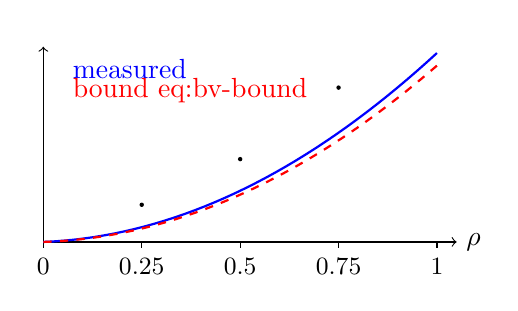
\begin{tikzpicture}[x=5cm, y=4cm]
    \draw[->] (0,0) -- (1.05,0) node[right] {$\rho$};
    \draw[->] (0,0) -- (0,0.62) node[above] {$\loss$};
    \foreach \t in {0,0.25,0.5,0.75,1} \draw (\t,0) -- (\t,-0.02) node[below] {\small $\t$};
    \draw[thick, blue, domain=0:1, samples=40] plot (\x, {0.55*\x*\x + 0.05*\x});
    \draw[thick, red, dashed, domain=0:1, samples=40] plot (\x, {0.52*\x*\x + 0.04*\x});
    \foreach \p/\q in {0.25/0.118, 0.5/0.263, 0.75/0.490} \fill (\p,\q) circle (0.8pt);
    \node[blue, anchor=west] at (0.05,0.55) {measured};
    \node[red, anchor=west] at (0.05,0.48) {bound \eqref{eq:bv-bound}};
  \end{tikzpicture}
  \caption{Loss as a function of the mask ratio (synthetic).}\label{fig:curve}
\end{figure}

\begin{figure}[htbp]
  \centering
  
\includegraphics[width=0.4\linewidth]{figures/heatmap}
  \caption{A synthetic reconstruction error map.}\label{fig:sample}
\end{figure}

\begin{theorem}\label{thm:monotone}
  Under \cref{lem:bias-variance}, the optimal loss is nondecreasing in $\rho$:
  \begin{equation}
    \rho \le \rho' \implies \min_W \Exp\mse[\mask_\rho]{W} \le \min_W \Exp\mse[\mask_{\rho'}]{W}.
    \label{eq:monotone}
  \end{equation}
\end{theorem}

\begin{remark}
  The gap in \cref{tab:ratios} grows roughly like $\rho^2$, consistent with
  \begin{align}
    \Delta(\rho) &\approx c\,\rho^2 + O(\rho^3), \notag \\
    \intertext{and with the fitted constant}
    c &= 0.03 \pm 0.01. \label{eq:fit}
  \end{align}
\end{remark}

\begin{enumerate}[label=(\roman*)]
  \item The bound is tight for linear models (\cref{eq:wstar}).
  \item It is loose by $\epsilon = \oldepsilon/2$ for attention models; see \citep{roe2022views,lee2024note}.
\end{enumerate}


\appendix
\section{Additional derivations}\label{app:derivations}

For completeness, the gradient of the linear loss is
\begin{equation}\label{eq:grad}
  \nabla_W \mse[\mask]{W} = -2\,\mask^\top\bigl(\mask\vx - \mask W \vis\vx\bigr)(\vis\vx)^\top ,
\end{equation}
and with a Gram matrix
\[
  G = \begin{pmatrix}
    \inp{\vx_1}{\vx_1} & \cdots & \inp{\vx_1}{\vx_n} \\
    \vdots & \ddots & \vdots \\
    \inp{\vx_n}{\vx_1} & \cdots & \inp{\vx_n}{\vx_n}
  \end{pmatrix} \succeq 0
\]
the empirical version of \eqref{eq:objective} is $\frac{1}{n}\sum_{i=1}^{n} \norm{\mask(\vx_i - W\vis\vx_i)}^2$.
Compare with \cref{thm:monotone} and \cref{sec:intro}.


\bibliographystyle{plainnat}
\bibliography{refs}

\end{document}
